\documentclass[luatex,fontsize=8pt,paper=b5,fleqn]{jlreq}
\usepackage{hyperref}
\usepackage{gckanbun}
\usepackage{luwa-ul}
\usepackage{caption}
\usepackage[most]{tcolorbox}
\usepackage{fp}
\usepackage{lltjext}
\usepackage{luatexja-ruby}
\usepackage{KKsymbols}

% You can omit these font settings.
\RequirePackage[no-math]{fontspec}
\RequirePackage[no-math,match,scale=1]{luatexja-fontspec}
\RequirePackage[hiragino-pro,deluxe,expert]{luatexja-preset}
\setmainfont{HiraMinPro-W3}[BoldFont=HiraMinPro-W6]\setmainjfont{HiraMinPro-W3}[BoldFont=HiraMinPro-W6]
\renewfontfamily{\sffamily}{HiraKakuPro-W3}[BoldFont=HiraKakuPro-W6]
\renewfontfamily{\mcfamily}{HiraMinPro-W3}[BoldFont=HiraMinPro-W6]
\renewfontfamily{\gtfamily}{HiraKakuPro-W3}[BoldFont=HiraKakuPro-W6]
\providefontfamily{\mgfamily}{HiraMaruPro-W4}
\newfontfamily{\sfhira}{HiraKakuPro-W3}[BoldFont=HiraKakuPro-W6]\newjfontfamily{\sfhiraj}{HiraKakuPro-W3}[BoldFont=HiraKakuPro-W6]
\newfontfamily{\mchira}{HiraMinPro-W3}[BoldFont=HiraMinPro-W6]\newjfontfamily{\mchiraj}{HiraMinPro-W3}[BoldFont=HiraMinPro-W6]
\newfontfamily{\gthira}{HiraKakuPro-W3}[BoldFont=HiraKakuPro-W6,FontFace={eb}{\shapedefault}{HiraKakuStd-W8}]\newjfontfamily{\gthiraj}{HiraKakuPro-W3}[BoldFont=HiraKakuPro-W6,FontFace={eb}{\shapedefault}{HiraKakuStd-W8}]
\newfontfamily{\mghira}{HiraMaruPro-W4}\newjfontfamily{\mghiraj}{HiraMaruPro-W4}
\renewcommand{\sffamily}{\sfhira\sfhiraj}
\renewcommand{\mcfamily}{\mchira\mchiraj}
\renewcommand{\gtfamily}{\gthira\gthiraj}
\renewcommand{\mgfamily}{\mghira\mghiraj}
%%%

\usepackage{listings}
\lstset{
    basicstyle=\ttfamily\small,
    keywordstyle=\color{blue},
    commentstyle=\color{gray},
    stringstyle=\color{red},
    breaklines=true,
    breakatwhitespace=false,  
    columns=flexible           
}


\usepackage{hyperref} 
\hypersetup{
  luatex, pdfencoding=auto, 
  colorlinks=true,
  linkcolor=black,     
  citecolor=black,     
  urlcolor=DeepSkyBlue3,      
  pdfborder={0 0 0}, 
}

\colorlet{grayLight}{white!80!black} 

\NewTCBListing{SourceCode}{ m m !o !O{DeepSkyBlue3} }{%
  enhanced, colback=black!70, colframe=Snow4,
  toptitle=-1mm, bottomtitle=-1mm,
  righttitle=-1mm, lefttitle=-1mm,
  arc=.5mm, 
  title={\tcbox[on line, arc=.5mm, boxsep=0pt, boxrule=0pt, top=1mm, bottom=0.8mm, left=2mm, right=2.2mm, colback=gray!80, coltext=white]{\raisebox{-0.1ex}{\vphantom{羅}\vphantom{j}#1}}},fonttitle=\gtfamily\footnotesize,boxrule=0.8pt,
  breakable,before upper={\color{white}},top=-0.5mm,bottom=-0.5mm,
  after title=\IfNoValueTF{#3}{}{{\hfill\tcbox[on line, arc=.5mm, boxsep=0pt, boxrule=0pt, top=1mm, bottom=0.8mm, left=2mm, right=2.2mm, colback=white!80!black, coltext=#4]{\raisebox{-0.1ex}{\vphantom{羅}\vphantom{j}#3}}}},
  listing only,
  listing options={
    language={#2},
    basicstyle=\ttfamily,
    keywordstyle=\ttfamily\color{white},
    stringstyle=\itshape\color{white},
    commentstyle=\small\gtfamily\color{DeepSkyBlue2},
    showspaces=false,showtabs=false,
    breaklines=true,breakindent=0pt,
    showstringspaces=false,
    columns=fullflexible,
    tabsize=2,
    numbers=left,numbersep=1.5pt,
    numberstyle=\scriptsize\gtfamily\color{gray},
  }
}

\NewTColorBox{OutPut}{ m !o !O{DeepSkyBlue3} }{%
  enhanced, colframe=Snow4,
  toptitle=-1mm, bottomtitle=-1mm,
  righttitle=-1mm, lefttitle=-1mm,
  arc=.5mm, colback=white, 
  fontupper=\normalsize,
  title={\tcbox[on line, arc=.5mm, boxsep=0pt, boxrule=0pt, top=1mm, bottom=0.8mm, left=2mm, right=2.2mm, colback=gray!40, coltext=DeepSkyBlue3]{\raisebox{-0.1ex}{\vphantom{羅}\vphantom{j}#1}}},fonttitle=\gtfamily\footnotesize,boxrule=0.8pt,
  breakable,top=-0.5mm,bottom=-0.5mm,
  after title=\IfNoValueTF{#2}{}{{\hfill\tcbox[on line, arc=.5mm, boxsep=0pt, boxrule=0pt, top=1mm, bottom=0.8mm, left=2mm, right=2.2mm, colback=white!80!black, coltext=#3]{\raisebox{-0.1ex}{\vphantom{羅}\vphantom{j}#2}}}}, bottom=2mm, top=2mm, 
}


\makeatletter
\RequirePackage{luatexja}
\def\ascb@textgt#1{\textgt{#1}}
\def\ascb@gtfamily{\gtfamily}
\def\ascb@zw#1#2{#1\zw}

\DeclareTColorBox{simple}{ o m O{.5} O{} }% 
{empty, left=2mm, right=2mm, top=-1mm, attach boxed title to top left={xshift=\ascb@zw{1.2}{11pt}}, boxed title style={empty,left=-2mm,right=-2mm}, colframe=black, coltitle=black, coltext=black, breakable, 
before upper={\setlength{\parindent}{1em}\relax},
underlay unbroken={\draw[black,line width=#3pt](title.east) -- (title.east-|frame.east) -- (frame.south east) -- (frame.south west) -- (title.west-|frame.west) -- (title.west); },
underlay first={\draw[black,line width=#3pt](title.east) -- (title.east-|frame.east) -- (frame.south east) ;
\draw[black,line width=#3pt] (frame.south west) -- (title.west-|frame.west) -- (title.west); },
underlay middle={\draw[black,line width=#3pt](frame.north east) -- (frame.south east) ;
\draw[black,line width=#3pt](frame.south west) -- (frame.north west) ;},
underlay last={\draw[black,line width=#3pt](frame.north east) -- (frame.south east) -- (frame.south west) -- (frame.north west) ;},
fonttitle=\ascb@gtfamily, IfValueTF={#1}{title=\hspace*{.1em}【#2】〈#1〉\hspace*{.1em}}{title=\hspace*{.1em}【#2】\hspace*{.1em}},#4}
\makeatother

\title{\texttt{gckanbun} Package Documentation (Reworked)}
\author{%
\parbox[r]{8cm}{%
  Original ver. : Munehiro Yamamoto\\
  Modified ver. : Kosei Kawaguchi a.k.a. KKTeX
}}
\date{Version 2.2.5 (2025/12/29)}


\begin{document}
\begin{titlepage}
  \maketitle
\end{titlepage}
\newpage
\tableofcontents
\newpage

\section{概要}
このリワークは、gckanbunパッケージを、日本における漢文組版においてより高い品質を担保できるように改変したものです。オリジナルの作者様である山本宗宏（Munehiro Yamamoto）さんとの協議により、メンテナーを形式上私川口晃世（KKTeX）が引き継ぐこととなりました。

gckanbunパッケージはそのルビや返り点の制御構造において非常に優れていたため、大枠はオリジナルのそれを踏襲し、必要最低限の拡張及び変更にとどめています。また、本パッケージに関する山本さんの記事として、
\begin{quotation}
  \url{https://qiita.com/munepi/items/5e6ac49fa5c025123305}
\end{quotation}
\noindent もぜひご参照ください。

\section{変更点}
私は本パッケージを作成するにあたり、既存のgckanbunパッケージを以下を満たすように改変しました。

\begin{itemize}
  \item[\seihou{1}] \hspace{1em}再読文字に対応するコマンドの提供。
  \item[\seihou{2}] \hspace{1em}横書き環境でも正しく動くようにする。
  \item[\seihou{3}] \hspace{1em}一レ点などの特別な返り点に対処するためのコマンドを提供する。
  \item[\seihou{4}] \hspace{1em}行間に対してルビの「大きさ」が反映されるように変更。（それに伴い、オリジナルで生じていた文字サイズ変更に伴うルビと本文の被りが生じる問題を解消。）
  \item[\seihou{5}] \hspace{1em}筆者の作成した（TeX Live にも収録されている）luwa-ul パッケージと併用し易い仕様にする。
\end{itemize}

\section{設置・依存性}
\subsection{読み込み}
適切な場所に\texttt{gckanbun.sty}のファイルを設置し、\verb|\usepackage{gckanbun}|とかけば読み込みは完了です。

本パッケージはLuaLaTeXでも(u)pLaTeXでも使用が可能です。

\subsection{オプション}
パッケージオプションは\verb|prefix=<prefix>|（デフォルト値：\verb|gckanbun|）となっていて、\texttt{gckanbun}パッケージが提供する3つのコマンド\verb|\gckanbunruby|、\verb|\gckanbunokurigana|、\verb|\gckanbunkaeriten| をそれぞれ\verb|<prefix>ruby|、\verb|<prefix>okurigana|、\verb|<prefix>kaeriten| として提供します。このオプションにより、他のパッケージで提供されるルビ振りコマンド \verb|\ruby| との衝突を避けられます。

\namiKK{以下の説明においては、\texttt{prefix}を空白として指定したものと仮定してコマンド名を表記しています。必要に応じて補って読んでください。}

\section{各種コマンド}
\subsection{概観}
漢文組版において必要十分であるコマンドは、

\begin{itemize}
  \item 返り点
  \item 振り仮名
  \item 送り仮名
  \item 再読振り仮名
  \item 再読送り仮名
  \item 一レ点、上レ点、甲レ点、天レ点
  \item ハイフン
\end{itemize}

\noindent です。これらに対し、本パッケージでは、それぞれ

\begin{itemize}
  \item \verb|\<prefix>kaeriten|、\verb|\返り|
  \item \verb|\<prefix>furigana|、\verb|\振り|
  \item \verb|\okurigana|、\verb|\送り|
  \item \verb|\<prefix>furigana|、\verb|\振り|のオプショナル引数
  \item \verb|\<prefix>okurigana|、\verb|\送り|のオプショナル引数
  \item \verb|\IchiRe|、\verb|\JyouRe|、\verb|\KouRe|、\verb|\TenRe|
  \item \verb|\KanHyphen|
\end{itemize}

\noindent が対応しています。

このうち、\texttt{prefix}が適用されるのは\verb|\<prefix>kaeriten|、\verb|\<prefix>furigana|、\verb|\<prefix>okurigana|のみであることに注意が必要です。

\subsection{使用方法}

\subsubsection{\textbackslash kaeriten、\textbackslash 返り}
これらの２種類のコマンドは全く同一のコマンドです。

\begin{SourceCode}{Input}{TeX}
  雖\返り{\IchiRe}鬼

  雖\返り{\JyouRe}鬼

  雖\返り{\KouRe}鬼

  雖\返り{\TenRe}鬼
\end{SourceCode}

\begin{OutPut}{Output}[横書き]
  雖\返り{\IchiRe}鬼

  雖\返り{\JyouRe}鬼

  雖\返り{\KouRe}鬼

  雖\返り{\TenRe}鬼
\end{OutPut}

のような出力になります。

\subsubsection{\textbackslash furigana、\textbackslash 振り、\textbackslash okurigana、\textbackslash 送り}

\verb|\furigana|、\verb|\振り|は同一、\verb|\okurigana|、\verb|\送り|は同一です。

\begin{SourceCode}{Input}{TeX}
  \振り{雖}{いへど}\送り{モ}\\
  \振り{所}{ゆ}\返り[intrusion=post]{二}\振り{\KanHyphen}{ゑ}\振り{以}{ん}\\
  \振り{猶}{な}[ごと]\送り{ホ}[キヲ]
\end{SourceCode}

\begin{OutPut}{Output}[横書き]
  \振り{雖}{いへど}\送り{モ}\\
  \振り{所}{ゆ}\返り[intrusion=post]{二}\振り{\KanHyphen}{ゑ}\振り{以}{ん}\\
  \振り{猶}{な}[ごと]\送り{ホ}[キヲ]
\end{OutPut}

v2.1.0以前では、各コマンドにはスターオプションがありましたが、現在では別の仕様に変更されました\footnote{以前は、スターオプションをつけると振り仮名や送り仮名の部分が行間計算に影響を与えなくなるという仕様を設けていましたが、使用されることがほぼないため削除しました。代わりに、\texttt{GCKEnv}の内部では（通常よりも行間を広く取ってあり、文字同士がぶつからない環境であるため）、行間が完全に揃うように自動的に適用されるようになりました。}。

ちなみに、「所以」のようなハイフンを含んだ熟語を打つ場合、\verb|\返り[intrusion=post]{二}|のように\verb|[intrusion=post]|のオプションを入れると出力は綺麗になります。

\section{局所縦書き}
このパッケージによって提供されるコマンドは局所的な縦書きにも対応しています（v2.2.0以降限定ですので、それ以前のものだと出力が壊れることに注意してください。）。

局所縦書きを開始する際には、\verb|\GCKTateOn|を入れます。もし、通常が縦書き環境の中で局所横書きをする場合には\verb|\GCKTateOff|となります。

\begin{SourceCode}{Input}{TeX}
  \parbox<t>{8\zw}{\GCKTateOn%
    \振り{雖}{いへど}\送り{モ}\\
    \振り{所}{ゆ}\返り[intrusion=post]{二}\振り{\KanHyphen}{ゑ}\振り{以}{ん}\\
    \振り{猶}{な}[ごと]\送り{ホ}[キヲ]
  \par}

  \parbox<t>{8\zw}{\GCKTateOn%
  今夫\送り{レ}江戸\振り{者}{は}、世之所\送り{ノ}\返り{レ}称\送り{スル}名都\振り{大}{だい}\振り{邑}{いふ}、%
  冠蓋之所\返り{レ}集\送り{マル}\LineNumbering*{\kakko{2}}\dashKK{舟車之\振り{所}{ところ}\送り{ニシテ}\返り{レ}\振り{湊}{あつ}\送り[intrusion=post]{マル}}、%
  実\送り{ニ}\振り{為}{た}\送り{ル}\返り{二}天下之大都会\返り{一}也。%
  而\送り{レドモ}\LineNumbering{C}\nolinebreak\underLineKKAuto{其地之為名、訪之於古、未之聞}。%
  豈\送り{二}非\送り{ズ}\返り{三}古今相\送り{ヒ}去\送り{ルコト}\振り{日}{ひび}\送り{ニ}遠\送り{ク}、%
  事之相\送り{ヒ}変\送り{ズルコト}愈多\送り{ク}、%
  求\送り{ムルモ}\返り{二}其\送り{ノ}所\送り{ヲ}\返り{\IchiRe}欲\送り{スル}\返り{レ}聞\送り{カント}而不\送り{ルコト}可\送り{カラ}\返り{レ}得、%
  亦\送り{タ}\振り{猶}{な}[ごと]\送り{ホ}[キヲ]\返り{二}今之於\送り{ケルガ}\返り{\JyouRe}古\送り{ニ}也。\par%
  }
\end{SourceCode}

\begin{OutPut}{Output}[局所縦書き]
  \parbox<t>{8\zw}{\GCKTateOn%
    \振り{雖}{いへど}\送り{モ}\\
    \振り{所}{ゆ}\返り[intrusion=post]{二}\振り{\KanHyphen}{ゑ}\振り{以}{ん}\\
    \振り{猶}{な}[ごと]\送り{ホ}[キヲ]
  \par}

  \parbox<t>{8\zw}{\GCKTateOn%
  今夫\送り{レ}江戸\振り{者}{は}、世之所\送り{ノ}\返り{レ}称\送り{スル}名都\振り{大}{だい}\振り{邑}{いふ}、%
  冠蓋之所\返り{レ}集\送り{マル}\LineNumbering*{\kakko{2}}\dashKKAuto{舟車之\振り{所}{ところ}\送り{ニシテ}\返り{レ}\振り{湊}{あつ}\送り[intrusion=post]{マル}}、%
  実\送り{ニ}\振り{為}{た}\送り{ル}\返り{二}天下之大都会\返り{一}也。%
  而\送り{レドモ}\LineNumbering{C}\nolinebreak\underLineKKAuto{其地之為名、訪之於古、未之聞}。%
  豈\送り{二}非\送り{ズ}\返り{三}古今相\送り{ヒ}去\送り{ルコト}\振り{日}{ひび}\送り{ニ}遠\送り{ク}、%
  事之相\送り{ヒ}変\送り{ズルコト}愈多\送り{ク}、%
  求\送り{ムルモ}\返り{二}其\送り{ノ}所\送り{ヲ}\返り{\IchiRe}欲\送り{スル}\返り{レ}聞\送り{カント}而不\送り{ルコト}可\送り{カラ}\返り{レ}得、%
  亦\送り{タ}\振り{猶}{な}[ごと]\送り{ホ}[キヲ]\返り{二}今之於\送り{ケルガ}\返り{\JyouRe}古\送り{ニ}也。\par%
  }
\end{OutPut}

\section{通常の漢文}
通常の漢文を打つ際には、

\begin{itemize}
  \item ルビはモノルビ仕様
  \item 必ず\verb|\振り|→\verb|\送り|→\verb|\返り|の順番にコマンドを配置
\end{itemize}

\noindent の２点に注意します。

縦書き環境における出力は以下のようになります。\namiKK{漢詩でなければ}、通常の文章と同様の打ち方で問題ありません。

漢文に傍線を引く場合、luwa-ulパッケージが最適です。自動でルビを検出し、下線を適切に持ち上げてくれます。詳しい仕様は、luwa-ulのマニュアルをご参照ください。

\begin{SourceCode}{Input}{TeX}
  \documentclass[luatex,fontsize=8pt,paper=b5,tate]{jlreq}
  \usepackage{luwa-ul,KKsymbols}
  \usepackage{gckanbun}

  \begin{document}
  
  今夫\送り{レ}江戸\振り{者}{は}、世之所\送り{ノ}\返り{レ}称\送り{スル}名都\振り{大}{だい}\振り{邑}{いふ}、冠蓋之所\返り{レ}集\送り{マル}\LineNumbering*{\kakko{2}}\dashKKAuto{舟車之\振り{所}{ところ}\送り{ニシテ}\返り{レ}\振り{湊}{あつ}\送り[intrusion=post]{マル}}、実\送り{ニ}\振り{為}{た}\送り{ル}\返り{二}天下之大都会\返り{一}也。
  而\送り{レドモ}\LineNumbering{C}\nolinebreak\underLineKKAuto{其地之為名、訪之於古、未之聞}。
  豈\送り{二}非\送り{ズ}\返り{三}古今相\送り{ヒ}去\送り{ルコト}\振り{日}{ひび}\送り{ニ}遠\送り{ク}、事之相\送り{ヒ}変\送り{ズルコト}愈多\送り{ク}、求\送り{ムルモ}\返り{二}其\送り{ノ}所\送り{ヲ}\返り{\IchiRe}欲\送り{スル}\返り{レ}聞\送り{カント}而不\送り{ルコト}可\送り{カラ}\返り{レ}得、亦\送り{タ}\振り{猶}{な}[ごと]\送り{ホ}[キヲ]\返り{二}今之於\送り{ケルガ}\返り{\JyouRe}古\送り{ニ}也。

  \end{document}
\end{SourceCode}

\begin{OutPut}{Output}[縦書き]
  \begin{center}
    \parbox<t>{12\zw}{\GCKTateOn%
      今夫\送り{レ}江戸\振り{者}{は}、世之所\送り{ノ}\返り{レ}称\送り{スル}名都\振り{大}{だい}\振り{邑}{いふ}、%
      冠蓋之所\返り{レ}集\送り{マル}\LineNumbering*{\kakko{2}}\dashKKAuto{舟車之\振り{所}{ところ}\送り{ニシテ}\返り{レ}\振り{湊}{あつ}\送り[intrusion=post]{マル}}、%
      実\送り{ニ}\振り{為}{た}\送り{ル}\返り{二}天下之大都会\返り{一}也。%
      而\送り{レドモ}\LineNumbering{C}\nolinebreak\underLineKKAuto{其地之為名、訪之於古、未之聞}。%
      豈\送り{二}非\送り{ズ}\返り{三}古今相\送り{ヒ}去\送り{ルコト}\振り{日}{ひび}\送り{ニ}遠\送り{ク}、%
      事之相\送り{ヒ}変\送り{ズルコト}愈多\送り{ク}、%
      求\送り{ムルモ}\返り{二}其\送り{ノ}所\送り{ヲ}\返り{\IchiRe}欲\送り{スル}\返り{レ}聞\送り{カント}而不\送り{ルコト}可\送り{カラ}\返り{レ}得、%
      亦\送り{タ}\振り{猶}{な}[ごと]\送り{ホ}[キヲ]\返り{二}今之於\送り{ケルガ}\返り{\JyouRe}古\送り{ニ}也。\par%
    }
  \end{center}
\end{OutPut}

\section{漢詩}

漢詩を打つ場合には、\verb|\makebox|と\verb|intrusion|オプションを使います。\verb|intrusion|オプションを指定すると、ルビ文字が親文字の幅を超えた時に前後の領域に「侵入」する形で配置されます。

しかし、漢文はほとんどの文字に何らかのルビが振られるため、普段から侵入を許可する仕様にするとかえって読みづらいです。したがって、本当に必要な時にだけこのオプションを使うべきです。

漢詩において、各句の最初と最後の字が水平方向に揃っていないと見栄えを損なってしまいます。そこで、gckanbunパッケージでは\verb|\makebox|と\verb|intrusion|オプションの組み合わせによって漢詩を組版することを推奨します。

\begin{description}
  \item[\texttt{\textbackslash 振り}] \verb|intrusion=pre/post/both| の３種類
  \item[\texttt{\textbackslash 送り}] \verb|intrusion=post/both| の２種類
  \item[\texttt{\textbackslash 返り}] \verb|intrusion=post/both| の２種類
\end{description}

\noindent が各コマンドで提供されるオプションであることに注意し、

\begin{SourceCode}{Input}{TeX}
  \makebox[9\zw][t]{%
    \振り[intrusion=pre]{春}{しゅん}\hfill%
    \振り{眠}{みん}\hfill%
    不\返り{レ}\hfill%
    \振り{覚}{おぼ}\送り{エ}\返り{レ}\hfill%
    \振り{暁}{あかつき}\送り[intrusion=post]{ヲ}%
  }

  \makebox[9\zw][t]{%
    \振り{処}{しょ}\hfill%
    \振り{処}{しょ}\hfill%
    聞\送り{ク}\返り{二}\hfill%
    \underLineKKAuto{\振り{啼}{てい}\hfill%
    鳥\送り{ヲ}\返り[intrusion=post]{一}}%
  }

  \makebox[9\zw][t]{%
    \振り{夜}{や}\hfill%
    \振り{来}{らい}\hfill%
    風\hfill%
    雨\送り{ノ}\hfill%
    声%
  }

  \makebox[9\zw][t]{%
    花\hfill%
    \振り{落}{お}\送り{ツルコト}\hfill%
    知\送り{ル}\hfill%
    \振り{多}{た}\hfill%
    \振り[intrusion=post]{少}{しょう}%
  }

  \end{document}
\end{SourceCode}

\begin{OutPut}{Output}[縦書き（漢詩）]
  \parbox<t>{12\zw}{\GCKTateOn%
    \makebox[9\zw][t]{%
      \振り[intrusion=pre]{春}{しゅん}\hfill%
      \振り{眠}{みん}\hfill%
      不\返り{レ}\hfill%
      \振り{覚}{おぼ}\送り{エ}\返り{レ}\hfill%
      \振り{暁}{あかつき}\送り[intrusion=post]{ヲ}%
    }

    \makebox[9\zw][t]{%
      \振り{処}{しょ}\hfill%
      \振り{処}{しょ}\hfill%
      聞\送り{ク}\返り{二}\hfill%
      \underLineKKAuto{\振り{啼}{てい}\hfill%
      鳥\送り{ヲ}\返り[intrusion=post]{一}}%
    }

    \makebox[9\zw][t]{%
      \振り{夜}{や}\hfill%
      \振り{来}{らい}\hfill%
      風\hfill%
      雨\送り{ノ}\hfill%
      声%
    }

    \makebox[9\zw][t]{%
      花\hfill%
      \振り{落}{お}\送り{ツルコト}\hfill%
      知\送り{ル}\hfill%
      \振り{多}{た}\hfill%
      \振り[intrusion=post]{少}{しょう}%
    }%
  }
\end{OutPut}

以上のように「漢字１文字ごとに\verb|\hfill|を挿入」することによって適切な空きを確保し、その上で句の最初の文字に（必要ならば）\verb|intrusion=pre|、最後の文字に\verb|intrusion=post|とします。ただし、たとえば「\verb|鳥\送り{ヲ}\返り{一}|」のような１まとまりにおいて、\verb|\送り|と\verb|\返り|の両方に対して\verb|intrusion=post|をつける必要はありません。「一番最後の」要素に対してのみ\verb|intrusion=post|をつければ十分です。

\section{GCKEnv}
v2.2.5以降、\verb|GCKEnv|という環境が新規追加されました。この環境は、本パッケージを用いて漢文を、完全に統一された行間、より広い字間のもとに組版するために設けられたものです。

この環境を使うか否かは、

\begin{simple}{GCKEnvの使い分け}
  \begin{description}
    \item[漢文以外の文章中に漢文を入れたい] この場合は環境を使うと逆に行間が壊れる可能性があり、絶対に使用してはいけません。
    \item[漢文だけを綺麗に組版したい時] 使うことが推奨されます。  
  \end{description}
\end{simple}

\noindent に従ってください。

構文は

\begin{SourceCode}{Input}{TeX}
  % 通常
  \begin{GCKEnv}[<baselineskip>][<kanjiskip>]
    <内容>
  \end{GCKEnv}

  % 漢詩を打つ時
  \begin{GCKEnv*}[<baselineskip>][<kanjiskip>]
    <内容>
  \end{GCKEnv*}
\end{SourceCode}

\noindent となります。

\begin{description}
  \item[<baselineskip>] 行間をどの程度にするか指定します。
  \item[<kanjiskip>] 字間をどの程度にするか指定します。 
\end{description}

\noindent 以上が各引数の説明ですが、具体例を見ていただく方が早いでしょう。

\begin{SourceCode}{Input}{TeX}
  \LARGE
  \begin{GCKEnv}{2\zw}
    今夫\送り{レ}江戸\振り{者}{は}、之所\送り{ノ}\返り{レ}称\送り{スル}名都\振り{大}{だい}\振り{邑}{いふ}、冠蓋之所\返り{レ}集\送り{マル}\LineNumbering*{\kakko{2}}\dashKKAuto[bottom=.5\zw]{舟車之\振り{所}{ところ}\送り{ニシテ}\返り{レ}\振り{湊}{あつ}\送り[intrusion=post]{マル}}、実\送り{ニ}\振り{為}{た}\送り{ル}\返り{二}天下之大都会\返り{一}也。
    而\送り{レドモ}\LineNumbering{C}\nolinebreak\underLineKKAuto{其地之為名、訪之於古、未之聞}。
    豈\送り{二}非\送り{ズ}\返り{三}古今相\送り{ヒ}去\送り{ルコト}\振り{日}{ひび}\送り{ニ}遠\送り{ク}、事之相\送り{ヒ}変\送り{ズルコト}愈多\送り{ク}、求\送り{ムルモ}\返り{二}其\送り{ノ}所\送り{ヲ}\返り{\IchiRe}欲\送り{スル}\返り{レ}聞\送り{カント}而不\送り{ルコト}可\送り{カラ}\返り{レ}得、亦\送り{タ}\振り{猶}{な}[ごと]\送り{ホ}[キヲ]\返り{二}今之於\送り{ケルガ}\返り{\JyouRe}古\送り{ニ}也。
  \end{GCKEnv}

  \bigskip

  \begin{GCKEnv*}{3\zw}
    \makebox[9\zw][t]{%
      \振り[intrusion=pre]{春}{しゅん}\hfill%
      \振り{眠}{みん}\hfill%
      不\返り{レ}\hfill%
      \振り{覚}{おぼ}\送り{エ}\返り{レ}\hfill%
      \振り{暁}{あかつき}\送り[intrusion=post]{ヲ}%
    }

    \makebox[9\zw][t]{%
      \振り{処}{しょ}\hfill%
      \振り{処}{しょ}\hfill%
      聞\送り{ク}\返り{二}\hfill%
      \underLineKKAuto{\振り{啼}{てい}\hfill%
      鳥\送り{ヲ}\返り[intrusion=post]{一}}%
    }

    \makebox[9\zw][t]{%
      \fbox{\振り{夜}{や}}\hfill%
      \振り{来}{らい}\hfill%
      風\hfill%
      雨\送り{ノ}\hfill%
      声%
    }

    \makebox[9\zw][t]{%
      \fbox{花}\hfill%
      \振り{落}{お}\送り{ツルコト}\hfill%
      知\送り{ル}\hfill%
      \振り{多}{た}\hfill%
      \振り{少}{しょう}%
    }
  \end{GCKEnv*}
\end{SourceCode}

\begin{OutPut}{Output}[縦書き]
  \begin{center}
    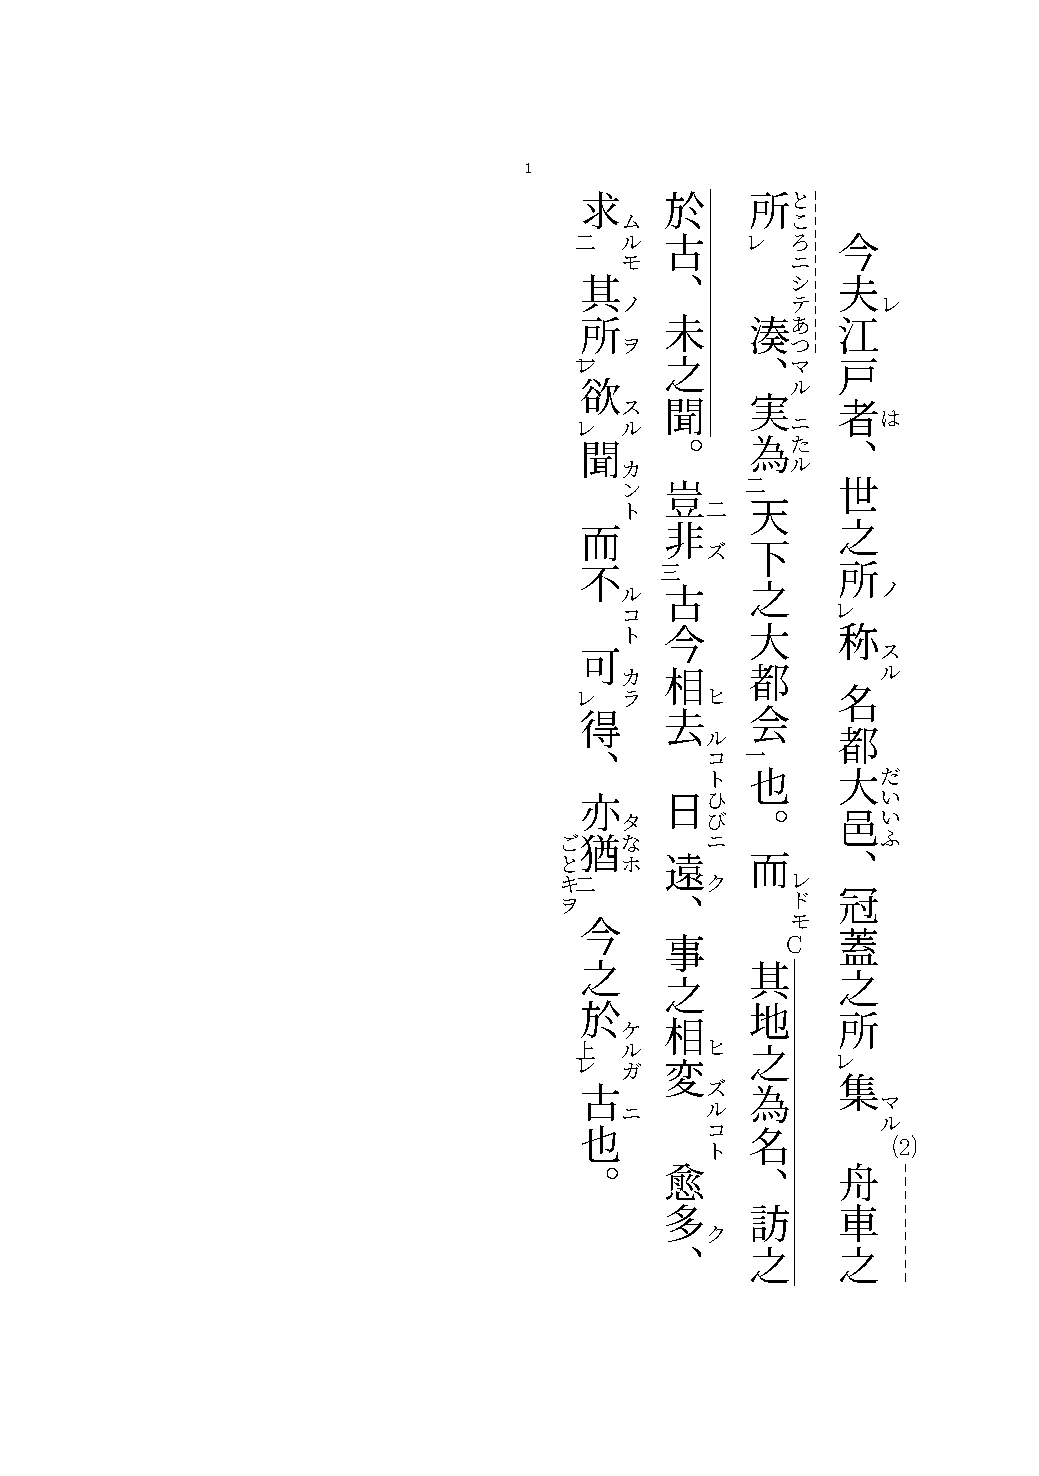
\includegraphics[width=.8\linewidth]{
      whole-vert-sample.pdf
    }
  \end{center}
\end{OutPut}

\section{ライセンス}
本パッケージをMITライセンスで配布します。条件なども全て以下のライセンス表記に準拠します。

\begin{simple}[gckanbun package]{ライセンス全文}\setlength{\parindent}{0em}%
  This package is licensed under the terms of the MIT License.

  Copyright (c) 2017-2025 Munehiro Yamamoto <munepixyz@gmail.com>\\
  Copyright (c) 2025 Kosei Kawaguchi

  Permission is hereby granted, free of charge, to any person obtaining a copy of this software and associated documentation files (the "Software"), to deal in the Software without restriction, including without limitation the rights to use, copy, modify, merge, publish, distribute, sublicense, and/or sell copies of the Software, and to permit persons to whom the Software is furnished to do so, subject to the following conditions:

  The above copyright notice and this permission notice shall be included in all copies or substantial portions of the Software.

  THE SOFTWARE IS PROVIDED "AS IS", WITHOUT WARRANTY OF ANY KIND, EXPRESS OR IMPLIED, INCLUDING BUT NOT LIMITED TO THE WARRANTIES OF MERCHANTABILITY, FITNESS FOR A PARTICULAR PURPOSE AND NONINFRINGEMENT. IN NO EVENT SHALL THE AUTHORS OR COPYRIGHT HOLDERS BE LIABLE FOR ANY CLAIM, DAMAGES OR OTHER LIABILITY, WHETHER IN AN ACTION OF CONTRACT, TORT OR OTHERWISE, ARISING FROM, OUT OF OR IN CONNECTION WITH THE SOFTWARE OR THE USE OR OTHER DEALINGS IN THE SOFTWARE.
\end{simple}


\section{Version History}
\begin{itemize}
  \item \textbf{v2.0.0 (2025/11/04)} --- Initial public release as a reworked version.
  \item \textbf{v2.1.0 (2025/11/12)} --- Modefied package documentation. Also, KKTeX added some options for KANSHI typesetting.
  \item \textbf{v2.2.0 (2025/12/26)} --- Fixed a problem in which a previous \verb|\送り| has an effect on the next \verb|\返り[intrusion=post]{arg}|. Also, make every commands can be used in partly-vertical-mode with the new \verb|\GCKTateOn|.
  \item \textbf{v2.2.1 (2025/12/28)} --- Eliminated every ex scale from .sty file.
  \item \textbf{v2.2.5 (2025/12/29)} --- Added \verb|GCKEnv| in order to typeset in more sophisticated way.
\end{itemize}

\section{Source Code}
\begin{lstlisting}
  \NeedsTeXFormat{LaTeX2e}
  \ProvidesPackage{gckanbun}[2025/12/29, Version 2.2.5]

  %% package errors
  \def\gcknbn@error{\PackageError{gckanbun}}
  \def\gcknbn@warning{\PackageWarning{gckanbun}}
  \def\gcknbn@warningnoline{\PackageWarningNoLine{gckanbun}}
  \def\gcknbn@info{\PackageInfo{gckanbun}}

  %% package options
  \RequirePackage{keyval,etoolbox}
  \DeclareOption*{\gcknbn@setkey}
  \def\gcknbn@setkey{\expandafter\@gcknbn@setkey\expandafter{\CurrentOption}}
  \def\@gcknbn@setkey{\setkeys{gcknbn}}
  \def\gcknbn@prefix{gckanbun}% given <prefix> for each commands
  \define@key{gcknbn}{prefix}{\gdef\gcknbn@prefix{#1}}

  \ExecuteOptions{prefix}
  \ProcessOptions\relax

  %% auto-detect engine
  \RequirePackage{ifuptex}
  \RequirePackage{ifluatex}
  \ifluatex
    \@ifpackageloaded{luatexja}{}{%
      \gcknbn@error{Please load package 'luatexja' when loading this package.}}
  \else\ifuptex
    \def\zw{zw}\def\zh{zh}
  \else\ifptex
    \def\zw{zw}\def\zh{zh}
  \else
    \gcknbn@error{Package 'gckanbun' currently supports (u)pLaTeX and LuaLaTeX.}
  \fi\fi\fi

  %% 縦書き判定
  \newif\ifgcknbn@tdir 
  \gcknbn@tdirfalse
  \@ifundefined{iftdir}{\let\iftdir\iffalse}{}%
  \ifluatex
    \@ifundefined{ltjgetparameter}{}{%
      \ifnum\ltjgetparameter{direction}=3 %
        \gcknbn@tdirtrue
      \fi}%
  \else
    \iftdir
      \gcknbn@tdirtrue
  \fi\fi

  %% kanjiskipの挿入
  \newcommand{\kanjiskip@gckanbun@env@post}{%
    \ifhmode
      % 1. 行頭（直前に何もノードがない状態）では何もしない
      % 2. または直前の空き(lastskip)が0より大きい場合のみ処理する
      \ifdim\lastskip > -1pt\relax % 行頭や特定の条件下では lastskip は 0 か特殊な値
        \unskip
        \hspace{\ltjgetparameter{kanjiskip}}\relax 
      \fi
    \fi
  }

  %% 縦書き補正、横書き補正を切り替える
  \newcommand{\GCKTateOn}{\gcknbn@tdirtrue}
  \newcommand{\GCKTateOff}{\gcknbn@tdirfalse}

  % 補正パラメータ
  \newlength{\gcknbn@adjust@yokotate}
  \NewDocumentCommand{\gcknbn@adjust@yokotate@use}{}{%
    \ifgcknbn@tdir
      \setlength{\gcknbn@adjust@yokotate}{-.7525\zw}%
    \else%
      \setlength{\gcknbn@adjust@yokotate}{-.56\zw}%
    \fi%
  }
  \newlength{\gcknbn@adjust@kaeri}
  \NewDocumentCommand{\gcknbn@adjust@kaeri@use}{}{%
    \ifgcknbn@tdir
      \setlength{\gcknbn@adjust@kaeri}{.35\zw}%
    \else%
      \setlength{\gcknbn@adjust@kaeri}{.15\zw}%
    \fi%
  }

  % phantom（再読文字分の行間を補正する）
  \def\gckanbun@phantom{\vphantom{あ}}

  %% ルビ
  %%  * グループルビ
  %%  * 漢文訓点に対するふりがな（モノルビ）
  \let\gcknbn@rubybox@text\relax
  \let\gcknbn@rubybox@text@s\relax
  \newdimen\gcknbn@rubybox@width
  \newdimen\gcknbn@furigana@width \gcknbn@furigana@width\z@
  \newdimen\gcknbn@furigana@width@s \gcknbn@furigana@width@s\z@
  \newdimen\gcknbn@dima

  % 侵入制御。
  % pre,post,bothをとれる。
  \newdimen\gcknbn@intr@pre
  \newdimen\gcknbn@intr@post
  \define@key{gcknbn@ruby}{intrusion}{\edef\gcknbn@ruby@intr@mark{#1}}
  \NewDocumentCommand{\gckanbun@intrusioncal}{}{%
    \ifdim\wd\@ne>\wd\tw@%侵入量計算
      \ifdim\wd\@ne>\zw%
        \global\gcknbn@intr@pre=\dimexpr(\wd\@ne-\zw)/2\relax%再読なし前方
        \global\gcknbn@intr@post=\dimexpr(\wd\@ne-\zw)/2\relax%再読なし後方
      \else%
        \global\gcknbn@intr@pre=0em\relax%
        \global\gcknbn@intr@post=0em\relax%
      \fi%
    \else%
      \ifdim\wd\tw@>\zw%
        \global\gcknbn@intr@pre=\dimexpr(\wd\tw@-\zw)/2\relax%再読あり前方
        \global\gcknbn@intr@post=\dimexpr(\wd\tw@-\zw)/2\relax%再読あり後方
      \else%
        \global\gcknbn@intr@pre=0em\relax%
        \global\gcknbn@intr@post=0em\relax%
      \fi%
    \fi%
  }

  % ルビ本体
  % 通常はsmashなしを使用。
  % Env内部のみsmashedに切り替わる。
  % 通常より行間を広く取れば、smashがあった方が行間が等しくなる。
  \DeclareDocumentCommand{\gcknbn@ruby}{ O{} m m O{\gckanbun@phantom}}{% normal
    \gcknbn@adjust@yokotate@use%
    \global\gcknbn@furigana@width\z@%
    \global\gcknbn@furigana@width@s\z@%
    \global\def\gcknbn@ruby@intr@mark{}%
    \leavevmode%
    \begingroup%
      \setkeys{gcknbn@ruby}{#1}%
      \gcknbn@dima\f@size\p@\relax \divide\gcknbn@dima by \tw@%
      \def\tiny{\@setfontsize\tiny{\gcknbn@dima}{\z@}}%
      \setbox\z@=\hbox{#2}% 親文字
      \setbox\@ne=\hbox{\tiny#3}% 振り仮名
      \setbox\tw@=\hbox{\tiny#4}% 再読振り仮名（通常はvphantomを入れている）
      \gckanbun@intrusioncal% 侵入量を計算
      \ifdefstring{\gcknbn@ruby@intr@mark}{pre}{%
        \kern-\gcknbn@intr@pre%
      }{%
        \ifdefstring{\gcknbn@ruby@intr@mark}{both}{%
          \kern-\gcknbn@intr@pre%
        }{%
          % それ以外は何もなし
      }}%
    \gdef\gcknbn@rubybox@text{#3}%
    \gdef\gcknbn@rubybox@text@s{#4}%
    \global\gcknbn@rubybox@width=\wd\z@\relax%
    \gcknbn@furigana@okurigana%
  }
  \DeclareDocumentCommand{\gcknbn@ruby@smashed}{ O{} m m O{\gckanbun@phantom}}{% smashed
    \kanjiskip@gckanbun@env@post%
    \gcknbn@adjust@yokotate@use%
    \global\gcknbn@furigana@width\z@%
    \global\gcknbn@furigana@width@s\z@%
    \global\def\gcknbn@ruby@intr@mark{}%
    \leavevmode%
    \begingroup%
      \setkeys{gcknbn@ruby}{#1}%
      \gcknbn@dima\f@size\p@\relax \divide\gcknbn@dima by \tw@%
      \def\tiny{\@setfontsize\tiny{\gcknbn@dima}{\z@}}%
      \setbox\z@=\hbox{#2}% 親文字
      \setbox\@ne=\hbox{\tiny#3}% 振り仮名
      \setbox\tw@=\hbox{\tiny#4}% 再読振り仮名（通常はvphantomを入れている）
      \gckanbun@intrusioncal% 侵入量を計算
      \ifdefstring{\gcknbn@ruby@intr@mark}{pre}{%
        \kern-\gcknbn@intr@pre%
      }{%
        \ifdefstring{\gcknbn@ruby@intr@mark}{both}{%
          \kern-\gcknbn@intr@pre%
        }{%
          % それ以外は何もなし
      }}%
    \gdef\gcknbn@rubybox@text{#3}%
    \gdef\gcknbn@rubybox@text@s{#4}%
    \global\gcknbn@rubybox@width=\wd\z@\relax%
    \gcknbn@furigana@okurigana@smashed%
  }

  % 次に来る文字を判定
  % 呼び出しを通常とsmashで変えている。
  \def\gcknbn@furigana@okurigana{% normal
    \futurelet\@let@token\gcknbn@@furigana@okurigana%
  }
  \def\gcknbn@furigana@okurigana@smashed{% smashed
    \futurelet\@let@token\gcknbn@@furigana@okurigana@smashed%
  }

  % 各種ボックスの長さを計算
  \NewDocumentCommand{\gckanbun@furigana@boxcal}{}{%
    \ifdim\wd\z@>\wd\@ne% \dimen\z@=max{\wd\z@,\wd\@ne,\wd\tw@}
      \dimen\z@=\wd\z@%
    \else%
      \dimen\z@=\wd\@ne%
    \fi%
    \ifdim\dimen\z@<\wd\tw@%
      \dimen\z@=\wd\tw@%
    \fi%
  }

  % ボックスの配置
  % 次が送り仮名の時
  \NewDocumentCommand{\gckanbun@furigana@boxing@nextokuri}{s}{%
    \IfBooleanTF{#1}{%
      \raisebox{\gcknbn@adjust@yokotate}{\smash{\hbox{%
        \vbox{\hbox to \dimen\z@{\box\@ne\hss}%
          \nointerlineskip\hbox to \dimen\z@{\hss\box\z@\hss}%
          \nointerlineskip\hbox to \dimen\z@{\box\tw@\hss}%
      }}}}%
    }{%
      \raisebox{\gcknbn@adjust@yokotate}{\hbox{%
        \vbox{\hbox to \dimen\z@{\box\@ne\hss}%
          \nointerlineskip\hbox to \dimen\z@{\hss\box\z@\hss}%
          \nointerlineskip\hbox to \dimen\z@{\box\tw@\hss}%
      }}}%
    }%
  }

  \newbox\gck@smashed@base
  \newbox\gck@smashed@furi
  \newdimen\gck@temp@h
  \newdimen\gck@temp@d
  % 次が送り仮名以外の時
  \NewDocumentCommand{\gckanbun@furigana@boxing@nextsonota}{s}{%
    \IfBooleanTF{#1}{%
    \setbox\gck@smashed@base\hbox{あ}%
    \edef\gck@temp@h{\the\ht\gck@smashed@base}%
    \edef\gck@temp@d{\the\dp\gck@smashed@base}%
    \setbox\gck@smashed@furi\hbox{%
      \raisebox{\gcknbn@adjust@yokotate}{\hbox{%
        \vbox{\hbox to \dimen\z@{\tiny\hss\gcknbn@rubybox@text\hss}%
          \nointerlineskip\hbox to \dimen\z@{\hss\box\z@\hss}%
          \nointerlineskip\hbox to \dimen\z@{\hss\box\tw@\hss}%
      }}}}%
    \ht\gck@smashed@furi=\gck@temp@h%
    \dp\gck@smashed@furi=\gck@temp@d%
    \box\gck@smashed@furi%
    }{%
      \raisebox{\gcknbn@adjust@yokotate}{\hbox{%
        \vbox{\hbox to \dimen\z@{\tiny\hss\gcknbn@rubybox@text\hss}%
          \nointerlineskip\hbox to \dimen\z@{\hss\box\z@\hss}%
          \nointerlineskip\hbox to \dimen\z@{\hss\box\tw@\hss}%
      }}}%
    }%
  }

  % 通常・再読振り仮名の長さをコピー
  % そして計算。
  \def\gckanbun@furigana@lenset{%
    \global\gcknbn@furigana@width=\wd\@ne\relax%
    \global\gcknbn@furigana@width@s=\wd\tw@\relax%
  }
  \newdimen\gcknbn@furigana@kutouten@kern
  \def\gcknbn@furigana@kutoten@skip{%
    \gcknbn@furigana@kutouten@kern=0pt\relax % リセット
    % どちらか一方が1\zwより大きいか
    \ifnum 0%
      \ifdim\gcknbn@furigana@width > 1\zw 1\fi%
      \ifdim\gcknbn@furigana@width@s > 1\zw 1\fi%
      > 0%
      %片方が1\zwを超えている場合
      \ifdim\gcknbn@furigana@width > \gcknbn@furigana@width@s%
        \gcknbn@furigana@kutouten@kern=\gcknbn@furigana@width%
      \else%
        \gcknbn@furigana@kutouten@kern=\gcknbn@furigana@width@s%
      \fi%
      \advance\gcknbn@furigana@kutouten@kern by -1\zw%
      \divide\gcknbn@furigana@kutouten@kern by \tw@%
    \fi%
    \hspace*{-\gcknbn@furigana@kutouten@kern}%
  }

  % 次のトークン（\@let@token）に応じて
  % 処理を切り替えている機構
  \def\gcknbn@@furigana@okurigana{% normal
    \ifx\@let@token\gcknbn@okurigana% 次が送り仮名の時
      \gckanbun@furigana@lenset%
      \dimen\z@=\wd\z@%
      \gckanbun@furigana@boxing@nextokuri%
    \else\ifx\@let@token、% 次が送り仮名ではない時
      \gckanbun@furigana@lenset%
      \gckanbun@furigana@boxcal%
      \penalty\@lowpenalty%
      \gckanbun@furigana@boxing@nextsonota%
      \gcknbn@furigana@kutoten@skip%
    \else\ifx\@let@token。%
      \gckanbun@furigana@lenset%
      \gckanbun@furigana@boxcal%
      \penalty\@lowpenalty%
      \gckanbun@furigana@boxing@nextsonota%
      \gcknbn@furigana@kutoten@skip%
    \else%
      \gckanbun@furigana@lenset%
      \gckanbun@furigana@boxcal%
      \penalty\@lowpenalty%
      \gckanbun@furigana@boxing@nextsonota%
    \fi\fi\fi%
    \ifdefstring{\gcknbn@ruby@intr@mark}{post}{%
      \kern-\gcknbn@intr@post%
    }{%
    \ifdefstring{\gcknbn@ruby@intr@mark}{both}{%
        \kern-\gcknbn@intr@post%
      }{%
        % それ以外は何もなし
    }}%
  \endgroup}
  \def\gcknbn@@furigana@okurigana@smashed{% smashed
    \ifx\@let@token\gcknbn@okurigana@smashed% 次が送り仮名の時
      \gckanbun@furigana@lenset%
      \dimen\z@=\wd\z@%
      \gckanbun@furigana@boxing@nextokuri*%
    \else\ifx\@let@token\gcknbn@kaeriten@smashed% 次が送り仮名ではない時
      \gckanbun@furigana@lenset%
      \gckanbun@furigana@boxcal%
      \penalty\@lowpenalty%
      \gckanbun@furigana@boxing@nextsonota*%
    \else\ifx\@let@token、%
      \gckanbun@furigana@lenset%
      \gckanbun@furigana@boxcal%
      \penalty\@lowpenalty%
      \gckanbun@furigana@boxing@nextsonota*%
      \kanjiskip@gckanbun@env@post%
      \gcknbn@furigana@kutoten@skip%
    \else\ifx\@let@token。%
      \gckanbun@furigana@lenset%
      \gckanbun@furigana@boxcal%
      \penalty\@lowpenalty%
      \gckanbun@furigana@boxing@nextsonota*%
      \kanjiskip@gckanbun@env@post%
      \gcknbn@furigana@kutoten@skip%
    \else%
      \gckanbun@furigana@lenset%
      \gckanbun@furigana@boxcal%
      \penalty\@lowpenalty%
      \gckanbun@furigana@boxing@nextsonota*%
      \kanjiskip@gckanbun@env@post%
    \fi\fi\fi\fi%
    \ifdefstring{\gcknbn@ruby@intr@mark}{post}{%
      \kern-\gcknbn@intr@post%
    }{%
    \ifdefstring{\gcknbn@ruby@intr@mark}{both}{%
        \kern-\gcknbn@intr@post%
      }{%
        % それ以外は何もなし
    }}%
  \endgroup}

  %% 訓点
  \newdimen\gcknbn@okurigana@width \gcknbn@okurigana@width\z@
  \newdimen\gcknbn@okurigana@width@s \gcknbn@okurigana@width@s\z@
  \newdimen\gcknbn@kaeriten@width \gcknbn@kaeriten@width\z@

  \define@key{gcknbn@okurigana}{intrusion}{\edef\gcknbn@okuri@intr@mark{#1}}
    % post,bothをとれるが挙動は一緒

  % 送り仮名のボックスを計算
  \NewDocumentCommand{\gckanbun@okurigana@boxcal}{}{%
    \ifdim\gcknbn@furigana@width>0.9999\zw\relax%
      \global\gcknbn@okurigana@width=\dimexpr\gcknbn@furigana@width + \wd\z@ - 1\zw\relax%
    \else%
      \global\gcknbn@okurigana@width=\dimexpr\wd\z@ - .5\zw\relax%
    \fi%
    \ifdim\gcknbn@furigana@width@s>0.9999\zw\relax%
      \global\gcknbn@okurigana@width@s=\dimexpr\gcknbn@furigana@width@s + \wd\@ne - 1\zw\relax%
    \else%
      \global\gcknbn@okurigana@width@s=\dimexpr\wd\@ne - .5\zw\relax%
    \fi%
  }

  % ボックスの配置
  \NewDocumentCommand{\gckanbun@okurigana@boxing}{s}{%
    \IfBooleanTF{#1}{%
      \smash{\hbox{%
          \raisebox{\gcknbn@adjust@yokotate}{\vbox{%
            \hbox to \gcknbn@okurigana@width{%
              \ifdim\gcknbn@furigana@width>0.9999\zw\relax%
                \hspace*{\dimexpr\gcknbn@furigana@width - 1\zw\relax}%
              \else%
                \hspace*{-.5\zw}%
              \fi%
              \box\z@}%
              \nointerlineskip%
              \hbox to \gcknbn@okurigana@width{%
                \hss%
                \vphantom{\char\euc"A1A1}%
                \hss%
              }%
              \nointerlineskip%
              \hbox to \gcknbn@okurigana@width@s{%
                \ifdim\gcknbn@furigana@width@s>0.9999\zw\relax%
                  \hspace*{\dimexpr\gcknbn@furigana@width@s - 1\zw\relax}%
                \else%
                  \hspace*{-.5\zw}%
                \fi%
                \box\@ne%
      }}}}}%
    }{%
      \hbox{%
        \raisebox{\gcknbn@adjust@yokotate}{%
          \vbox{\hbox to \gcknbn@okurigana@width{%
            \ifdim\gcknbn@furigana@width>0.9999\zw\relax%
              \hspace*{\dimexpr\gcknbn@furigana@width - 1\zw\relax}%
            \else%
              \hspace*{-.5\zw}%
            \fi%
            \box\z@}%
            \nointerlineskip%
            \hbox to \gcknbn@okurigana@width{%
              \hss%
              \vphantom{\char\euc"A1A1}%
              \hss%
            }%
            \nointerlineskip%
            \hbox to \gcknbn@okurigana@width@s{%
              \ifdim\gcknbn@furigana@width@s>0.9999\zw\relax%
                \hspace*{\dimexpr\gcknbn@furigana@width@s - 1\zw\relax}%
              \else%
                \hspace*{-.5\zw}%
              \fi%
              \box\@ne%
      }}}}%
    }%
  }

  % 送り仮名本体
  \DeclareDocumentCommand{\gcknbn@okurigana}{ O{} m O{\gckanbun@phantom} }{% normal
    \nobreak\leavevmode%
    \gcknbn@adjust@yokotate@use%
    \global\gcknbn@okurigana@width\z@%
    \global\gcknbn@okurigana@width@s\z@%
    \global\def\gcknbn@okuri@intr@mark{}%
    \begingroup%
      \setkeys{gcknbn@okurigana}{#1}%
      \gcknbn@dima\f@size\p@\relax \divide\gcknbn@dima by \tw@%
      \def\tiny{\@setfontsize\tiny{\gcknbn@dima}{\z@}}%
      \setbox\z@=\hbox{\tiny #2}% 通常送り仮名
      \setbox\@ne=\hbox{\tiny #3}% 再読送り仮名（通常はvphantomを入れている）
      \gckanbun@okurigana@boxcal%
      \gckanbun@okurigana@boxing%
    \global\gcknbn@furigana@width=\z@\relax%
    \gcknbn@okurigana@intr%
    \gcknbn@okurigana@kaeriten%
  }
  \DeclareDocumentCommand{\gcknbn@okurigana@smashed}{ O{} m O{\gckanbun@phantom} }{% smashed
    \nobreak\leavevmode%
    \gcknbn@adjust@yokotate@use%
    \global\gcknbn@okurigana@width\z@%
    \global\gcknbn@okurigana@width@s\z@%
    \global\def\gcknbn@okuri@intr@mark{}%
    \begingroup%
      \setkeys{gcknbn@okurigana}{#1}%
      \gcknbn@dima\f@size\p@\relax \divide\gcknbn@dima by \tw@%
      \def\tiny{\@setfontsize\tiny{\gcknbn@dima}{\z@}}%
      \setbox\z@=\hbox{\tiny #2}% 通常送り仮名
      \setbox\@ne=\hbox{\tiny #3}% 再読送り仮名（通常はvphantomを入れている）
      \gckanbun@okurigana@boxcal%
      \gckanbun@okurigana@boxing*%
    \global\gcknbn@furigana@width=\z@\relax%
    \gcknbn@okurigana@intr%
    \gcknbn@okurigana@kaeriten@smashed%
  }

  % 次に来る文字をセット
  \def\gcknbn@okurigana@kaeriten{\futurelet\@let@token\gcknbn@@okurigana@kaeriten}
  \def\gcknbn@okurigana@kaeriten@smashed{\futurelet\@let@token\gcknbn@@okurigana@kaeriten@smashed}

  % 次に来るトークン毎に処理を変更
  \def\gcknbn@@okurigana@kaeriten{%
    \ifx\@let@token、
      \gcknbn@okurigana@kutoten@skip
      \global\gcknbn@okurigana@width=\z@
    \else\ifx\@let@token。
      \gcknbn@okurigana@kutoten@skip
      \global\gcknbn@okurigana@width=\z@
    \else\ifx\@let@token\gcknbn@kaeriten
      \gcknbn@okurigana@kaeriten@skip
    \else%
      \ifdefstring{\gcknbn@okuri@intr@mark}{post}{%
        \kern-\gcknbn@intr@post%
      }{%
      \ifdefstring{\gcknbn@okuri@intr@mark}{both}{%
          \kern-\gcknbn@intr@post%
        }{%
          % それ以外は何もなし
      }}%
    \fi\fi\fi
  \endgroup}
  \def\gcknbn@@okurigana@kaeriten@smashed{%
    \ifx\@let@token、%
      \gcknbn@okurigana@kutoten@skip%
      \kanjiskip@gckanbun@env@post%
      \global\gcknbn@okurigana@width=\z@%
    \else\ifx\@let@token。%
      \gcknbn@okurigana@kutoten@skip%
      \kanjiskip@gckanbun@env@post%
      \global\gcknbn@okurigana@width=\z@%
    \else\ifx\@let@token\gcknbn@kaeriten@smashed%
      \gcknbn@okurigana@kaeriten@skip%
    \else%
      \kanjiskip@gckanbun@env@post%
      \ifdefstring{\gcknbn@okuri@intr@mark}{post}{%
        \kern-\gcknbn@intr@post%
      }{%
      \ifdefstring{\gcknbn@okuri@intr@mark}{both}{%
          \kern-\gcknbn@intr@post%
        }{%
          % それ以外は何もなし
      }}%
    \fi\fi\fi
  \endgroup}

  % 各場合毎に入れるスペース
  \def\gcknbn@okurigana@kutoten@skip{%
    \ifdim\gcknbn@okurigana@width>\gcknbn@okurigana@width@s%
      \hspace*{-\gcknbn@okurigana@width}%
    \else%
      \hspace*{-\gcknbn@okurigana@width@s}%
    \fi%
  }
  \def\gcknbn@okurigana@kaeriten@skip{%
    \ifdim\gcknbn@okurigana@width>\gcknbn@okurigana@width@s%
      \hspace*{-\gcknbn@okurigana@width}%
    \else%
      \hspace*{-\gcknbn@okurigana@width@s}%
    \fi
  }
  \def\gcknbn@okurigana@intr{%
    \ifdim\gcknbn@okurigana@width>\gcknbn@okurigana@width@s%
      \global\gcknbn@intr@post=\gcknbn@okurigana@width%
    \else%
      \global\gcknbn@intr@post=\gcknbn@okurigana@width@s%
    \fi
  }

  %%訓点返り点
  \define@key{gcknbn@kaeriten}{intrusion}{\edef\gcknbn@kaeri@intr@mark{#1}}
    % post,bothをとれるが挙動は一緒

  % 返り点本体
  \DeclareDocumentCommand{\gcknbn@kaeriten}{ O{} m }{% normal
    \nobreak\leavevmode%
    \gcknbn@adjust@kaeri@use%
    \global\def\gcknbn@kaeri@intr@mark{}%
    \setkeys{gcknbn@kaeriten}{#1}%
    \begingroup%
      \gcknbn@dima\f@size\p@\relax \divide\gcknbn@dima by \tw@
      \def\tiny{\@setfontsize\tiny{\gcknbn@dima}{\z@}}%
      \setbox\z@=\hbox{\tiny #2}%
      \global\gcknbn@kaeriten@width=\wd\z@\relax
      \ifdim\wd\z@>\gcknbn@intr@post%
        \global\gcknbn@intr@post=\wd\z@%
      \fi%
      \lower\gcknbn@adjust@kaeri\hbox{\box\z@\hss}%
    \endgroup%
    \gcknbn@kaeriten@kutoten%
  }
  \DeclareDocumentCommand{\gcknbn@kaeriten@smashed}{ O{} m }{% smashed
    \nobreak\leavevmode%
    \gcknbn@adjust@kaeri@use%
    \global\def\gcknbn@kaeri@intr@mark{}%
    \setkeys{gcknbn@kaeriten}{#1}%
    \begingroup%
      \gcknbn@dima\f@size\p@\relax \divide\gcknbn@dima by \tw@
      \def\tiny{\@setfontsize\tiny{\gcknbn@dima}{\z@}}%
      \setbox\z@=\hbox{\tiny #2}%
      \global\gcknbn@kaeriten@width=\wd\z@\relax
      \ifdim\wd\z@>\gcknbn@intr@post%
        \global\gcknbn@intr@post=\wd\z@%
      \fi%
      \smash{\lower\gcknbn@adjust@kaeri\hbox{\box\z@\hss}}%
    \endgroup%
    \gcknbn@kaeriten@kutoten@smashed%
  }

  % 次に来る文字をセット
  \def\gcknbn@kaeriten@kutoten{\futurelet\@let@token\gcknbn@@kaeriten@kutoten}
  \def\gcknbn@kaeriten@kutoten@smashed{\futurelet\@let@token\gcknbn@@kaeriten@kutoten@smashed}

  % 次に来る文字毎に処理を変更
  \def\gcknbn@@kaeriten@kutoten{%
    \ifx\@let@token、%
      \gcknbn@kaeriten@kutoten@skip%
      \global\gcknbn@kaeriten@width=\z@%
    \else\ifx\@let@token。%
      \gcknbn@kaeriten@kutoten@skip%
      \global\gcknbn@kaeriten@width=\z@%
    \else%
      \ifdefstring{\gcknbn@kaeri@intr@mark}{post}{%
        \kern-\gcknbn@intr@post%
      }{%
      \ifdefstring{\gcknbn@kaeri@intr@mark}{both}{%
          \kern-\gcknbn@intr@post%
        }{%
          \gcknbn@kaeriten@okurigana@skip%
      }}%
    \fi\fi%
  }
  \def\gcknbn@@kaeriten@kutoten@smashed{%
    \ifx\@let@token、%
      \gcknbn@kaeriten@kutoten@skip%
      \global\gcknbn@kaeriten@width=\z@%
    \else\ifx\@let@token。%
      \gcknbn@kaeriten@kutoten@skip%
      \global\gcknbn@kaeriten@width=\z@%
    \else%
      \kanjiskip@gckanbun@env@post%
      \ifdefstring{\gcknbn@kaeri@intr@mark}{post}{%
        \kern-\gcknbn@intr@post%
      }{%
      \ifdefstring{\gcknbn@kaeri@intr@mark}{both}{%
          \kern-\gcknbn@intr@post%
        }{%
          \gcknbn@kaeriten@okurigana@skip%
      }}%
    \fi\fi%
  }

  % 各場合分け毎に入れるスペース
  \def\gcknbn@kaeriten@kutoten@skip{%
    \ifgcknbn@tdir%
      \hspace*{-\gcknbn@kaeriten@width}%
    \fi%
  }
  \def\gcknbn@kaeriten@okurigana@skip{%
    \ifdim\gcknbn@okurigana@width>\gcknbn@kaeriten@width%
      \hspace*{\dimexpr\gcknbn@okurigana@width - \gcknbn@kaeriten@width}%
    \fi%
    \ifdim\gcknbn@okurigana@width<\gcknbn@okurigana@width@s%
      \hspace*{\gcknbn@okurigana@width@s - \gcknbn@kaeriten@width}%
    \else%
    \fi%
  }

  %% \<prefix>ruby, \<prefix>okurigana, \<prefix>kaeriten
  \expandafter\let\csname\gcknbn@prefix ruby\endcsname\gcknbn@ruby
  \expandafter\let\csname\gcknbn@prefix okurigana\endcsname\gcknbn@okurigana
  \expandafter\let\csname\gcknbn@prefix kaeriten\endcsname\gcknbn@kaeriten

  %% 短縮マクロ
  \expandafter\let\csname 振り\endcsname\gcknbn@ruby
  \expandafter\let\csname 送り\endcsname\gcknbn@okurigana
  \expandafter\let\csname 返り\endcsname\gcknbn@kaeriten

  %% 特殊返り点
  \NewDocumentCommand{\IchiRe}{}{%
    \ifgcknbn@tdir%
      \hspace{-0.21\zw}一\hspace{-0.72\zw}レ%
    \else%
      \raisebox{0.29\zw}{一}\llap{レ}%
    \fi%
  }
  \NewDocumentCommand{\JyouRe}{}{%
    \ifgcknbn@tdir%
      上\hspace{-0.3\zw}レ%
    \else%
      \raisebox{0.71\zw}{上}\llap{レ}%
    \fi%
  }
  \NewDocumentCommand{\KouRe}{}{%
    \ifgcknbn@tdir%
      甲\hspace{-0.17\zw}レ%
    \else%
      \raisebox{0.82\zw}{甲}\llap{レ}%
    \fi%
  }
  \NewDocumentCommand{\TenRe}{}{%
    \ifgcknbn@tdir%
      天\hspace{-0.17\zw}レ%
    \else%
      \raisebox{0.82\zw}{天}\llap{レ}%
    \fi%
  }
  \NewDocumentCommand{\KanHyphen}{}{\symbol{"2015}}


  %% GCKEnv
  \NewDocumentEnvironment{GCKEnv}{ m O{0.3\zw plus 0.15\zw minus 0.2\zw} }{%
    \ltjsetparameter{kanjiskip=#2}% ここもLuaのみの書き方になっているので注意。
    \setlength{\baselineskip}{#1}%
    \expandafter\let\csname\gcknbn@prefix ruby\endcsname\gcknbn@ruby@smashed%
    \expandafter\let\csname\gcknbn@prefix okurigana\endcsname\gcknbn@okurigana@smashed%
    \expandafter\let\csname\gcknbn@prefix kaeriten\endcsname\gcknbn@kaeriten@smashed%
    \expandafter\let\csname 振り\endcsname\gcknbn@ruby@smashed%
    \expandafter\let\csname 送り\endcsname\gcknbn@okurigana@smashed%
    \expandafter\let\csname 返り\endcsname\gcknbn@kaeriten@smashed%
  }{\par}
  \NewDocumentEnvironment{GCKEnv*}{ m O{0.3\zw plus 0.15\zw minus 0.2\zw} }{%
    \ltjsetparameter{kanjiskip=#2}% ここもLuaのみの書き方になっているので注意。
    \setlength{\baselineskip}{#1}%
  }{\par}

  \endinput
\end{lstlisting}

\end{document}